\section{Evaluation}\label{sec:evaluation}

% \begin{table*}[!t]
% \centering
% \caption{Answer generation quality of our \name{} and the baselines on the \textit{Academia} network. \textit{SP} means Shortest Paths, and \textit{CSP} refers to Constrained Shortest Paths. The win rates sum over 100\% as we allow multiple winners. \textbf{Bold faces} denote the highest win rate.}
% \label{tab:quality_academia}
% \resizebox{\textwidth}{!}{%
% \begin{tabular}{@{}clrrrrrrr@{}}
% \toprule
% \multirow{2}{*}{\textbf{Question Type}} & \multirow{2}{*}{\textbf{Criteria}} & \textbf{MS\_GraphRAG} & \textbf{RoG} & \textbf{Fast-graphrag} & \textbf{Graph-CoT} & \multirow{2}{*}{\textbf{Top-k SP}} & \multirow{2}{*}{\textbf{Top-k CSP}} & \multirow{2}{*}{\textbf{\name{}}} \\
%  &  & (BFS) & (Guided Walk) & (PPR) & (CoT) &  &  &  \\ \midrule
% \multirow{4}{*}{\textbf{$\langle s,*,*\rangle $}} & Comprehensiveness & \textbf{95.00\%} & N/A & 28.75\% & 21.25\% & N/A & N/A & \textbf{95.00\%} \\
%  & Diversity & \textbf{88.75\%} & N/A & 22.50\% & 15.00\% & N/A & N/A & \textbf{88.75\%} \\
%  & Empowerment & \textbf{85.00\%} & N/A & 32.50\% & 17.50\% & N/A & N/A & \textbf{85.00\%} \\
%  & Overall & \textbf{86.25\%} & N/A & 5.00\% & 8.75\% & N/A & N/A & \textbf{86.25\%} \\ \midrule
% \multirow{7}{*}{\textbf{$\langle s,p,*\rangle $}} & Comprehensiveness & 31.25\% & \textbf{80.00\%} & 31.25\% & 30.00\% & N/A & N/A & \textbf{80.00\%} \\
%  & Diversity & 23.75\% & \textbf{75.00\%} & 21.25\% & 7.50\% & N/A & N/A & \textbf{75.00\%} \\
%  & Empowerment & 30.00\% & \textbf{75.00\%} & 20.00\% & 7.50\% & N/A & N/A & \textbf{75.00\%} \\
%  & Overall & 23.75\% & \textbf{70.00\%} & 17.50\% & 6.25\% & N/A & N/A & \textbf{70.00\%} \\ \cmidrule(l){2-9} 
%  & Precision & 0.2 & \textbf{0.78} & 0.37 & 0.63 & N/A & N/A & \textbf{0.78} \\
%  & Recall & 0.17 & \textbf{0.76} & 0.29 & 0.44 & N/A & N/A & \textbf{0.76} \\
%  & F1 & 0.18 & \textbf{0.76} & 0.3 & 0.48 & N/A & N/A & \textbf{0.76} \\ \midrule
% \multirow{4}{*}{\textbf{$\langle s,*,o\rangle $}} & Comprehensiveness & 36.25\% & N/A & 0.00\% & 12.50\% & \textbf{93.75\%} & 18.75\% & \textbf{93.75\%} \\
%  & Diversity & 10.00\% & N/A & 0.00\% & 6.25\% & \textbf{92.50\%} & 16.25\% & \textbf{92.50\%} \\
%  & Empowerment & 21.25\% & N/A & 0.00\% & 5.00\% & \textbf{91.25\%} & 15.00\% & \textbf{91.25\%} \\
%  & Overall & 2.50\% & N/A & 0.00\% & 1.25\% & \textbf{88.75\%} & 10.00\% & \textbf{88.75\%} \\ \midrule
% \multirow{4}{*}{\textbf{$\langle s,p,o\rangle $}} & Comprehensiveness & 16.25\% & N/A & 16.25\% & 21.25\% & 35.00\% & \textbf{81.25\%} & \textbf{81.25\%} \\
%  & Diversity & 16.25\% & N/A & 10.00\% & 6.25\% & 42.50\% & \textbf{76.25\%} & \textbf{76.25\%} \\
%  & Empowerment & 11.25\% & N/A & 11.25\% & 7.50\% & 35.00\% & \textbf{83.75\%} & \textbf{83.75\%} \\
%  & Overall & 8.75\% & N/A & 3.75\% & 3.75\% & 22.50\% & \textbf{72.50\%} & \textbf{72.50\%} \\ \midrule
% \multicolumn{2}{c}{\textbf{Overall}} & 30.31\% & 17.50\% & 6.56\% & 5.00\% & 27.81\% & 20.63\% & \textbf{79.38\%} \\ \bottomrule
% \end{tabular}%
% }
% \end{table*}

In this part, we conduct experiments to evaluate \name{} and compare it with existing baseline solutions. 
% Through the experimental results, we tend to explore:

% \squishlist
% \item \textit{How well does \name{} generates responses to various graph questions compared to baselines?}

% \item \textit{How efficient is \name{} when answering various graph questions compared to baselines?}

% \item \textit{How many fewer tokens does \name{} consume to answer the question compared to baselines?}
% \squishend


\begin{table}[!t]
\caption{Response generation quality and efficiency of our \name{} and the baselines on \benchmarkname{}. The win rates sum over 100\% as we allow multiple winners for each question. \textbf{Bold faces} denote the best results. F1-score and Hit are only for $\langle s,p,* \rangle$ and $\langle s,p,* \rangle + \langle s,p,* \rangle$ questions.}
\label{tab:main_results}
\resizebox{\textwidth}{!}{%
\begin{tabular}{@{}llcccccc@{}}
\toprule
\multicolumn{2}{l}{\textbf{Criteria}} & \textbf{MS\_GraphRAG} & \textbf{RoG} & \textbf{Fast-graphrag} & \textbf{Graph-CoT} & \textbf{Cypher} & \textbf{PolyG} \\ \midrule
\multirow{9}{*}{\raisebox{-4em}{\rotatebox[origin=c]{90}{Claude-3.5-sonnet}}} & Comprehensiveness & 26.08\% & 28.75\% & 17.17\% & 19.42\% & 13.25\% & \textbf{74.67\%} \\
 & Diversity & 19.00\% & 26.33\% & 10.67\% & 15.83\% & 8.25\% & \textbf{66.08\%} \\
 & Empowerment & 24.42\% & 26.25\% & 15.83\% & 13.58\% & 12.67\% & \textbf{64.83\%} \\
 & Directness & 29.83\% & 15.75\% & 31.83\% & 42.42\% & 15.50\% & \textbf{46.67\%} \\
 & Overall Winner & 17.17\% & 19.25\% & 12.25\% & 13.83\% & 7.92\% & \textbf{54.75\%} \\ \cmidrule(l){2-8} 
 & F1-score & 0.2094 & 0.6934 & 0.3304 & 0.3885 & 0.1750 & \textbf{0.7084} \\
 & Hit & 0.4400 & 0.8867 & 0.6500 & 0.6500 & 0.3300 & \textbf{0.8900} \\ \cmidrule(l){2-8} 
 & Latency (s) & \textbf{11.79} & 16.75 & 45.84 & 53.81 & 14.84 & 25.38 \\
 & Token Usage & 17,464 & \textbf{1,417} & 48,038 & 104,594 & 4,273 & 6,950 \\ \midrule \midrule
\multirow{9}{*}{\raisebox{-3em}{\rotatebox[origin=c]{90}{Deepseek-R1}}} & Comprehensiveness & 29.17\% & 30.00\% & 33.08\% & 9.17\% & 22.83\% & \textbf{62.83\%} \\
 & Diversity & 24.00\% & 24.00\% & 29.67\% & 4.17\% & 14.92\% & \textbf{56.75\%} \\
 & Empowerment & 29.75\% & 25.50\% & 31.00\% & 4.08\% & 20.42\% & \textbf{50.58\%} \\
 & Directness & 33.00\% & 22.33\% & 36.58\% & 25.17\% & 29.83\% & \textbf{43.75\%} \\
 & Overall Winner & 21.92\% & 21.83\% & 24.17\% & 5.08\% & 17.50\% & \textbf{42.92\%} \\ \cmidrule(l){2-8} 
 & F1-score & 0.3246 & 0.6048 & 0.4752 & 0.2952 & 0.2835 & \textbf{0.6153} \\
 & Hit & 0.4400 & 0.6767 & 0.7000 & 0.3867 & 0.3533 & \textbf{0.6867} \\ \cmidrule(l){2-8} 
 & Latency (s) & \textbf{13.50} & 17.05 & 46.76 & 93.02 & 23.03 & 22.40 \\
 & Token Usage & 16,843 & \textbf{1,534} & 48,038 & 86,128 & 5,014 & 5,796 \\ \bottomrule
\end{tabular}%
}
\end{table}


\subsection{Experiment Setting}

We compare \name{} against several baselines: MS\_GraphRAG~\cite{ms_graphrag}, RoG~\cite{rog}, Fast-graphrag~\cite{fast_graphrag}, and Graph-CoT~\cite{graphcot}, on \benchmarkname{}. Additionally, we include a baseline named \textit{Cypher}, which directly generates Cypher queries using the LLM without guidance from our proposed question pattern taxonomy to show the necessity of our adaptive prompting. To evaluate performance, we follow the evaluation practices of previous work~\cite{ms_graphrag, lightrag}, assessing generation quality based on win rates judged by the LLM across five dimensions: \textit{Comprehensiveness}, \textit{Diversity}, \textit{Empowerment}, \textit{Directness}, and \textit{Overall Winner}. Following previous works, we also report \textit{F1-score} and \textit{Hit} on the questions having golden ground-truth, namely of the type $\langle s,p,* \rangle$ and $\langle s,p,* \rangle + \langle s,p,* \rangle$, along with \textit{response latency} and \textit{token usage} as efficiency metrics. We evaluate the main results using both Claude-3.5-sonnet~\cite{claude} and Deepseek-R1~\cite{deepseekr1} for generation, and Deepseek-R1 to give judgments. For ablation studies and micro-benchmarks, we provide the results with Claude-3.5-sonnet. Detailed experimental settings are provided in~\autoref{sec:exp_settings_appendix}.


\subsection{Experiment Results}

\stitle{Main results.} \autoref{tab:main_results} presents the generation quality and execution efficiency across all three knowledge graphs in \benchmarkname{}. In terms of generation quality, \name{} consistently achieves the highest win rates across all four evaluation criteria, with the most overall wins, as well as the highest F1-score and Hit. These results highlight the limitations of existing GraphRAG methods and underscore the importance of adaptive graph traversal in handling diverse graph questions. The superior performance of \name{} on both Claude-3.5-sonnet and Deepseek-R1 suggests its generalization across different LLMs. RoG achieves comparable quantitative scores to \name{}, as it is specifically tailored for $\langle s,p,* \rangle$ questions. While Graph-CoT is generally applicable to any question type due to the reasoning flexibility of LLMs, its win rates are lower because the LLM often explores only a subset of relevant entities and derives answers from a limited view of the knowledge graph. This results in less comprehensive and diverse responses compared to methods that retrieve all relevant entities. However, this narrow focus allows Graph-CoT to perform comparably to \name{} in terms of directness.


In terms of execution efficiency and cost (see \autoref{tab:main_results}), \name{} achieves superior generation quality without a significant increase in response latency or token usage. Instead, it maintains relatively low latency and substantially reduces token consumption compared to more resource‐intensive baselines. Specifically, \name{} consistently records lower latency and requires fewer tokens than Fast-GraphRAG and Graph-CoT. This efficiency arises because Fast-GraphRAG relies on dynamic computation of Personalized PageRank (PPR) scores for each node during retrieval, and Graph-CoT invokes the LLM at every traversal step—both of which incur high computational complexity and resource usage. MS\_GraphRAG also exhibits high token consumption by retrieving large amounts of irrelevant information, even when questions target specific aspects. Although RoG and Cypher offer shorter latency and lower token usage, they do not match \name{}’s generation quality, which remains the primary criterion for GraphRAG applications.



\begin{table}[!t]
\centering
\caption{Win rates for each of the basic question patterns and nested questions.}
\label{tab:overall_decompose}
\resizebox{0.95\textwidth}{!}{%
\begin{tabular}{@{}ccccccc@{}}
\toprule
\textbf{Question Pattern} & \textbf{MS\_GraphRAG} & \textbf{RoG} & \textbf{Fast-graphrag} & \textbf{Graph-CoT} & \textbf{Cypher} & \textbf{PolyG} \\ \midrule
$\langle s,*,* \rangle$ & 30.00\% & 23.75\% & 2.92\% & 26.25\% & 15.00\% & \textbf{33.33\%} \\
$\langle s,p,* \rangle$ & 10.83\% & \textbf{47.08\%} & 24.58\% & 18.33\% & 13.33\% & 45.00\% \\
$\langle s,*,o \rangle$ & 25.83\% & 9.17\% & 5.42\% & 10.00\% & 3.75\% & \textbf{59.58\%} \\
$\langle s,p,o \rangle$ & 4.17\% & 1.25\% & 20.42\% & 5.83\% & 3.75\% & \textbf{70.42\%} \\
Nested & 15.00\% & 15.00\% & 7.92\% & 8.75\% & 3.75\% & \textbf{65.42\%} \\ \bottomrule
\end{tabular}%
}
% \vspace{-2mm}
\end{table}


\stitle{Response quality for different question patterns.} In~\autoref{tab:overall_decompose}, we break down the win rate by the four basic question patterns and nested questions. We observe that some baselines achieve win rates comparable to \name{} on $\langle s, *, * \rangle$ (e.g., MS\_GraphRAG) and $\langle s, p, * \rangle$ (e.g., RoG) questions. For the $\langle s, *, * \rangle$ pattern, questions are typically simple and seek general information about entities; MS\_GraphRAG is specifically designed and well-optimized for such tasks. RoG achieves similar win rates to \name{} on $\langle s, p, * \rangle$ questions because this pattern is the primary focus of existing KGQA benchmarks targeted by RoG. Consequently, similar performance trends are also observed on representative KGQA benchmarks, where \name{} matches RoG and outperforms all other baselines. Although specific baselines perform similarly to \name{} in terms of the “\textit{Overall Winner}” metric for these two question patterns, \name{} outperforms them in other criteria (e.g., \textit{Comprehensiveness}), making it a preferable choice for users with specific priorities. For all other patterns, \name{} constantly delivers superior response quality, achieving overall win rates above 60\%.

\begin{figure}[!t]
    \centering
    \begin{subfigure}[b]{0.48\textwidth}
        \centering
        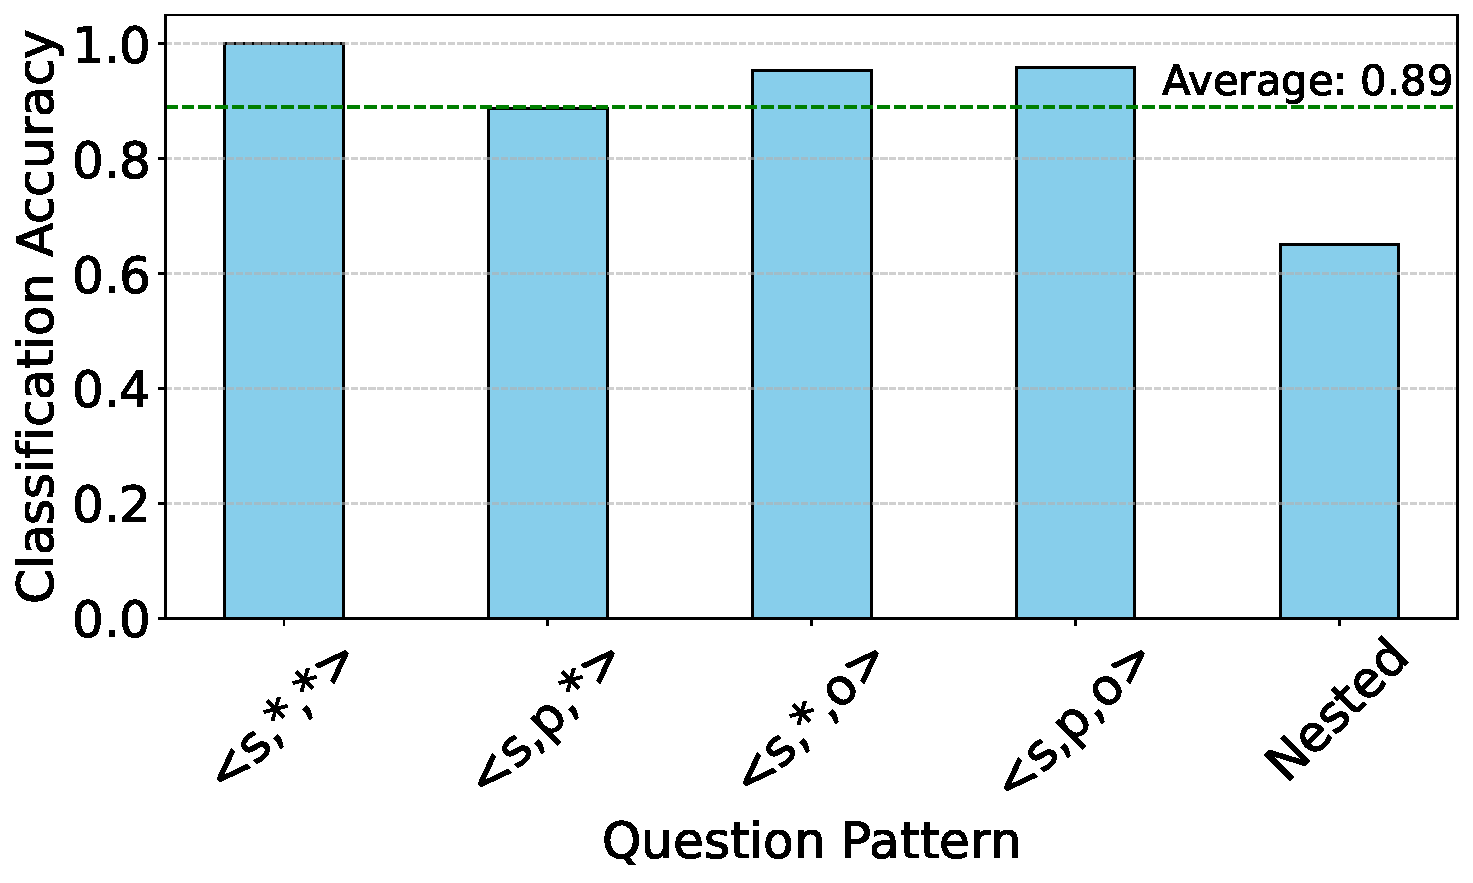
\includegraphics[width=\textwidth]{figures/exp/qc_accuracy.pdf}
        \caption{Accuracy of question categorization.}
        \label{fig:qc_acc}
    \end{subfigure}
    % \hfill
    \begin{subfigure}[b]{0.48\textwidth}
        \centering
        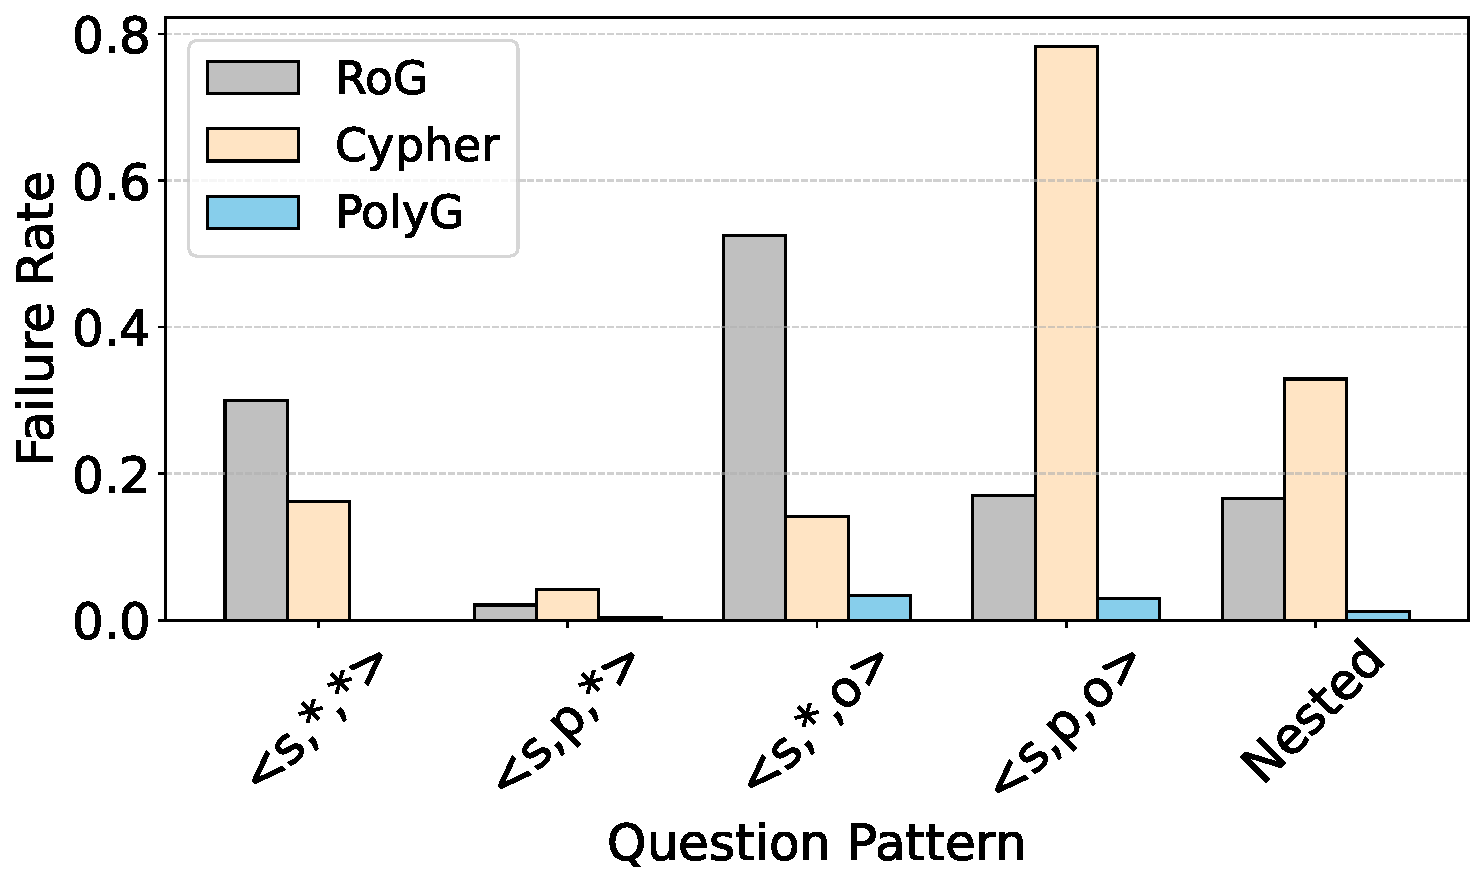
\includegraphics[width=\textwidth]{figures/exp/failure_rate.pdf}
        \caption{Failure rate comparison.}
        \label{fig:failure_rate}
    \end{subfigure}
    \caption{Question categorization accuracy and failure rates of \name{} on each question pattern.}
    \label{fig:micro_exp}
    % \vspace{-4mm}
\end{figure}

\stitle{Accuracy of question categorization.} \autoref{fig:qc_acc} presents the accuracy of LLM-based question categorization in \name{} for different question patterns. The average accuracy is 89\%, demonstrating that our question pattern taxonomy is clear and effective for the LLM to differentiate between the patterns. Notably, accuracy is lower for $\langle s, p, * \rangle$ and nested questions compared to the other three patterns. This is because \name{} tends to decompose complex $\langle s, p, * \rangle$ questions involving multi-hop relations into multiple steps, while it merges simple nested questions of the form $\langle s, p, * \rangle + \langle s, p, * \rangle$ into a single $\langle s, p, * \rangle$ question. However, such decomposition and merging do not impair the LLM’s ability to generate quality responses, and thus we allow this intrinsic flexibility.


\stitle{Failure analysis.} Although the LLM is provided with the graph schema in \name{}, it can still generate incorrect Cypher queries—either semantically incorrect or returning empty results. To evaluate the effectiveness of our self-correction module during Cypher query generation, we report the failure rates broken down by the 4 basic and nested question patterns in~\autoref{fig:failure_rate}. For comparison, we also include the failure rates of RoG and Cypher. The results show that \name{} successfully generates correct Cypher queries for over 95\% of the questions, while RoG and Cypher fail for 24\% and 30\% of tasks, respectively. Furthermore, without the LLM self-correction module, \name{} would fail for 70\% of the nested questions. These findings suggest that our adaptive prompting and self-correction mechanism effectively reduce failures and enable more reliable Cypher query generation.


\stitle{Additional experiments.} In~\autoref{sec:result_decompose_appendix}, we provide additional experimental results. These include win rate decompositions across the other four criteria, detailed performance and efficiency comparisons on each dataset, and further analysis of the nested question pattern.


% \begin{table*}[!t]
% \centering
% \caption{End-to-end generation latency (s) and  total token usage of \name{} and the baselines on all 3 datasets. The results are in the form \textit{time/tokens}. \textit{SP} stands for Shortest Paths, and \textit{CSP} refers to Constrained Shortest Paths.}
% \label{tab:time_token}
% \resizebox{\textwidth}{!}{%
% \begin{tabular}{@{}ccrrrrrrr@{}}
% \toprule
% \multirow{2}{*}{\textbf{Dataset}} & \multirow{2}{*}{\textbf{Question Type}} & \textbf{MS\_GraphRAG} & \textbf{RoG} & \textbf{Fast-graphrag} & \textbf{Graph-CoT} & \multirow{2}{*}{\textbf{Top-k SP}} & \multirow{2}{*}{\textbf{Top-k CSP}} & \multirow{2}{*}{\textbf{\name{}}} \\
%  &  & (BFS) & (Guided Walk) & (PPR) & (CoT) &  &  &  \\ \midrule
% \multirow{4}{*}{\textbf{Academia}} & $\langle s,*,*\rangle $ & 10.25/8,412 & N/A & 32.84/73,041 & 41.67/30,767 & N/A & N/A & 11.01/8,931 \\
%  & $\langle s,p,*\rangle $ & 5.13/7,789 & 11.33/1,127 & 28.18/64,816 & 44.14/42,352 & N/A & N/A & 12.11/1,651 \\
%  & $\langle s,*,o\rangle $ & 7.6/13,352 & N/A & 28.78/72,218 & 57.11/48,929 & 25.5/1,107 & 16.21/1,346 & 26.31/1,640 \\
%  & $\langle s,p,o\rangle $ & 77.84/44,637 & N/A & 27.42/55,738 & 72.14/164,723 & 9.89/661 & 19.46/1,873 & 20.24/2,406 \\ \midrule
% \multirow{4}{*}{\textbf{Literature}} & $\langle s,*,*\rangle $ & 9.06/4,209 & N/A & 19.89/25,427 & 50.5/43,983 & N/A & N/A & 9.86/4,723 \\
%  & $\langle s,p,*\rangle $ & 4.73/1,682 & 13.05/1,517 & 18.39/28,706 & 56.66/68,211 & N/A & N/A & 13.88/2,037 \\
%  & $\langle s,*,o\rangle $ & 8.63/13,277 & N/A & 17.54/28,853 & 49.21/43,498 & 6.43/1,021 & 13.52/1,225 & 7.24/1,548 \\
%  & $\langle s,p,o\rangle $ & 29.32/58,673 & N/A & 19.5/38,960 & 108.01/448,029 & 6.48/607 & 16.31/1,733 & 17.10/2,269 \\ \midrule
% \multirow{4}{*}{\textbf{E-commerce}} & $\langle s,*,*\rangle $ & 7.82/6,885 & N/A & 64.79/61,330 & 44.34/36,018 & N/A & N/A & 8.65/7,406 \\
%  & $\langle s,p,*\rangle $ & 5.36/7,040 & 11.59/1,357 & 59.77/41,113 & 50.58/54,298 & N/A & N/A & 12.39/1,885 \\
%  & $\langle s,*,o\rangle $ & 7.84/17,523 & N/A & 58.73/45,560 & 52.06/54,464 & 6.32/1,428 & 12.85/1,204 & 7.14/1,971 \\
%  & $\langle s,p,o\rangle $ & 16.2/40,325 & N/A & 59.74/39,660 & 83.24/239,014 & 6.17/840 & 16.7/1,980 & 17.49/2,517 \\ \midrule
% \multicolumn{2}{c}{\textbf{Overall}} & 15.82/18,650 & 11.99/1,334 & 36.30/47,952 & 59.14/106,191 & 10.13/944 & 15.84/1,560 & 13.62/3,249 \\ \bottomrule
% \end{tabular}%
% }
% \end{table*}

% \begin{table}[!t]
% \caption{End-to-end generation latency (s) and total token usage of \name{} and the baselines on all 3 datasets.}
% \label{tab:time_token}
% \resizebox{\textwidth}{!}{%
% \begin{tabular}{@{}ccrrrrrr@{}}
% \toprule
% \multirow{2}{*}{\textbf{Dataset}} & \multirow{2}{*}{\textbf{Metric}} & \textbf{MS\_GRAG} & \textbf{RoG} & \textbf{Fast-grag} & \textbf{Graph-CoT} & \multirow{2}{*}{\textbf{Text2Cypher}} & \multirow{2}{*}{\textbf{\name{}}} \\
%  &  & (BFS) & (Guided Walk) & (PPR) & (CoT) & & \\ \midrule
% \multirow{2}{*}{Phyics}    & Time  & 13.18  & 16.04       & 29.62  & 52.85   & 13.64          & 33.68  \\
%                            & Token & 13,523 & 1,507       & 67,963 & 78,185  & 5,763          & 10,260 \\ \midrule
% \multirow{2}{*}{Goodreads} & Time  & 12.6   & 16.21       & 17.9   & 63.31   & 12.08          & 34.62  \\
%                            & Token & 17,976 & 1,570       & 30,446 & 146,845 & 3,970          & 10,711 \\ \midrule
% \multirow{2}{*}{Amazon}    & Time  & 10.55  & 17.68       & 62.62  & 59.38   & 14.83          & 24.01  \\
%                            & Token & 21,150 & 1,591       & 45,708 & 96,533  & 5,068          & 6,868  \\ \bottomrule
% \end{tabular}
% }
% \end{table}

% \stitle{End-to-end latency.} \autoref{tab:time_token} presents the end-to-end response latency of \name{} and baseline methods across all three knowledge graphs. ``N/A'' indicates that a method is not applicable to the corresponding question type. The latency of \name{} includes the execution time of the selected traversal method plus the overhead of LLM-based question categorization. In some cases, \name{} exhibits higher latency than BFS and Top-$k$ SP, as these methods retrieve less relevant context and yield lower win rates (see \autoref{tab:quality_academia} and \autoref{tab:quality_literature}). Consequently, \name{} selects more effective traversal methods, such as Guided Walk and Top-$k$ CSP, to ensure better context retrieval. Additionally, \name{} consistently outperforms PPR and CoT, as PPR requires dynamically computing PPR scores for each node during retrieval, and CoT invokes the LLM at every step of graph traversal—both incurring high computational complexity and resource consumption. Furthermore, BFS can also be inefficient in certain cases of the $\langle s, p, o \rangle$ question type due to the inherent skewness of graphs, where expanding all neighbors of a high-degree entity significantly increases computational cost.


% \stitle{Token consumption.} 
% \autoref{tab:time_token} also reports the total number of tokens consumed by \name{} and each baseline method. The token consumption of \name{} includes both the tokens required for answering a specific question type and the additional overhead from prompting the LLM to classify the question into one of the four predefined types. Results show that \name{} achieves the best generation quality while requiring the least number of tokens in most cases. There are instances where certain baseline methods consume fewer tokens than \name{}, such as Top-$k$ SP for the $\langle s, p, o \rangle$ question type. This occurs because Top-$k$ SP retrieves the shortest paths between the two given entities, whereas \name{} selects the Top-$k$ CSP method, which retrieves only the shortest reasoning paths that satisfy the relation constraint in the question. These paths are typically longer than those retrieved by Top-$k$ SP. Despite its lower token usage, Top-$k$ SP underperforms in generation quality, as it retrieves paths that focus on other relationships rather than those specified in the query, leading to less informative responses.

% \begin{table}[!t]
% \centering
% \caption{Question categorization overhead of \name{} on all 4 question types and 3 datasets.}
% \label{tab:overhead}
% \resizebox{0.85\columnwidth}{!}{%
% \begin{tabular}{cccc}
% \hline
% \textbf{Dataset} & \textbf{Question Type} & \textbf{Time (s)} & \textbf{Tokens} \\ \hline
% \multirow{4}{*}{\textbf{Academia}} & \textbf{$\langle s, p_a, ?\rangle $} & 0.76 & 518.99 \\
%  & \textbf{$\langle s, p_c, ?\rangle $} & 0.78 & 523.94 \\
%  & \textbf{$\langle s, ?_a, o\rangle $} & 0.81 & 532.98 \\
%  & \textbf{$\langle s, ?_c, o\rangle $} & 0.78 & 533.05 \\ \hline
% \multirow{4}{*}{\textbf{Literature}} & \textbf{$\langle s, p_a, ?\rangle $} & 0.80 & 514.31 \\
%  & \textbf{$\langle s, p_c, ?\rangle $} & 0.83 & 520.43 \\
%  & \textbf{$\langle s, ?_a, o\rangle $} & 0.81 & 526.88 \\
%  & \textbf{$\langle s, ?_c, o\rangle $} & 0.79 & 535.59 \\ \hline
% \multirow{4}{*}{\textbf{E-commerce}} & \textbf{$\langle s, p_a, ?\rangle $} & 0.83 & 521.29 \\
%  & \textbf{$\langle s, p_c, ?\rangle $} & 0.80 & 527.83 \\
%  & \textbf{$\langle s, ?_a, o\rangle $} & 0.82 & 542.78 \\
%  & \textbf{$\langle s, ?_c, o\rangle $} & 0.79 & 536.85 \\ \hline
% \end{tabular}%
% }
% \end{table}


% \begin{figure}[!t]
% 	\centering
% 	\includegraphics[width=0.8\columnwidth]{figures/exp/scatter_quality_time.pdf}
% 	% \vspace{-2mm}
% 	\caption{Overall comparison for \name{} and the baselines on generation quality (\%) end end-to-end generation latency (s).}
% 	\label{fig:quality_time}
% 	\vspace{-4mm}
% \end{figure}

% \stitle{Result summary.} 
% \autoref{fig:quality_time} provides an overall comparison of \name{} and baseline methods in terms of both generation quality and system efficiency, averaged across the three datasets. The results indicate that baseline methods exhibit low average win rates across all four question types, suggesting that relying on a fixed traversal method does not perform well across diverse graph questions. In particular, Fast-GraphRAG and Graph-CoT incur high computational costs in their traversal operations, leading to prolonged end-to-end response latency. In contrast, by dynamically selecting an appropriate traversal method for each question type, \name{} achieves the highest win rate while maintaining low end-to-end latency, demonstrating the necessity of question categorization and adaptive graph traversal.

